\section{Måger (vildtkending og biologi)}

% ========== TITEL: MÅGEFUGLE ==========
\begin{frame}
  \vspace{1.5em}
  \begin{center}
    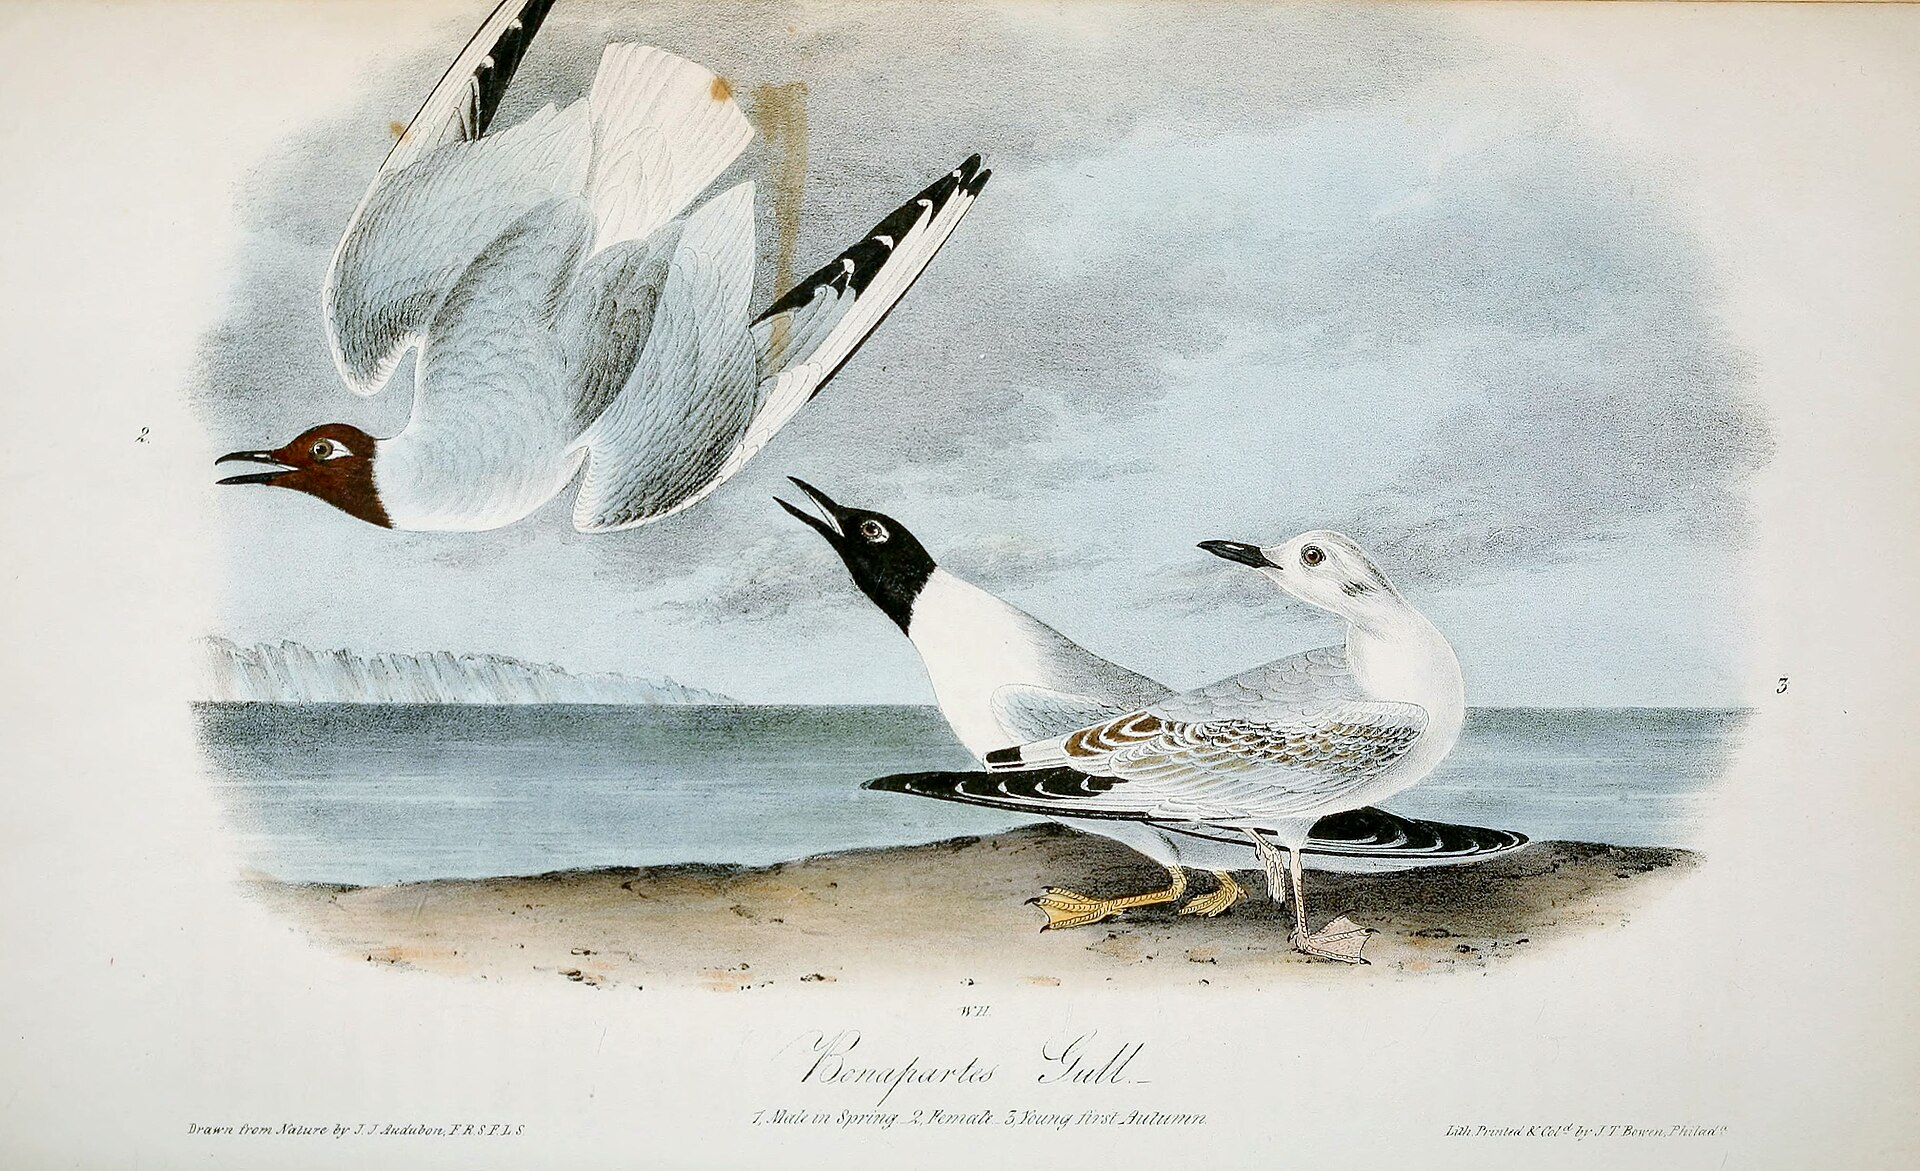
\includegraphics[width=12cm, height=4cm, keepaspectratio]{Billeder/Dyr/Fugle/Mågefugle/maagefugle.jpg}\\[1.2em]
    {\LARGE \textbf{Mågefugle}}\\[0.6em]
   
    Artsbestemmelse \& vildtbiologi\\[0.9em]
    {\tiny\color{gray}
    CC BY 4.0 – kan frit anvendes, også kommercielt. Rettighederne må ikke skærpes.\\[0.05em]
    Udviklet af Aleksander Sønder, OSJAGTTEGN.DK}
  \end{center}
\end{frame}



% ========== SØLVMÅGE ==========
\begin{frame}{%
  \begin{minipage}[c]{0.30\textwidth}
    Sølvmåge
  \end{minipage}%
  \hfill
  \begin{minipage}[c]{0.45\textwidth}
    \footnotesize
    \textbf{Jagttid:} 1.\ september -- 31.\ januar*
  \end{minipage}%
  \hfill
  \begin{minipage}[c]{0.15\textwidth}
    \noindent\raggedleft
    
\includegraphics[width=0.5cm, height=0.5cm, keepaspectratio]{Billeder/Ikoner/star.png}%
    \hspace{0.2em}%
    
\includegraphics[width=0.5cm, height=0.5cm, keepaspectratio]{Billeder/Ikoner/star.png}
  \end{minipage}%
}
  \vspace{0.25em}
  \begin{columns}[T]
    \column{0.45\textwidth}
    \setlength{\parskip}{0.5em}
    \tiny
    \RaggedRight
    \textbf{\textit{Larus argentatus}} – stor og kraftig måge med flad isse \par
    \textbf{Udseende:}\\
    \quad – Grå ryg og vinger med sort vingespids \\
    \quad – Lyserøde ben \\
    \quad – Gult næb med rød plet på undernæbbets spids \par
    \textbf{Levesteder:} Ses overalt, hvor der er føde. \par
    \textbf{Føde:} Altædende. \par
    \textbf{Udbredelse:} Hele Danmark. \par
    \textbf{Træk/standfugl:} Standfugl \par
    \textbf{*Bemærk:} I flere østdanske kommuner først fra 1.\ november.
    \column{0.52\textwidth}
    \centering
    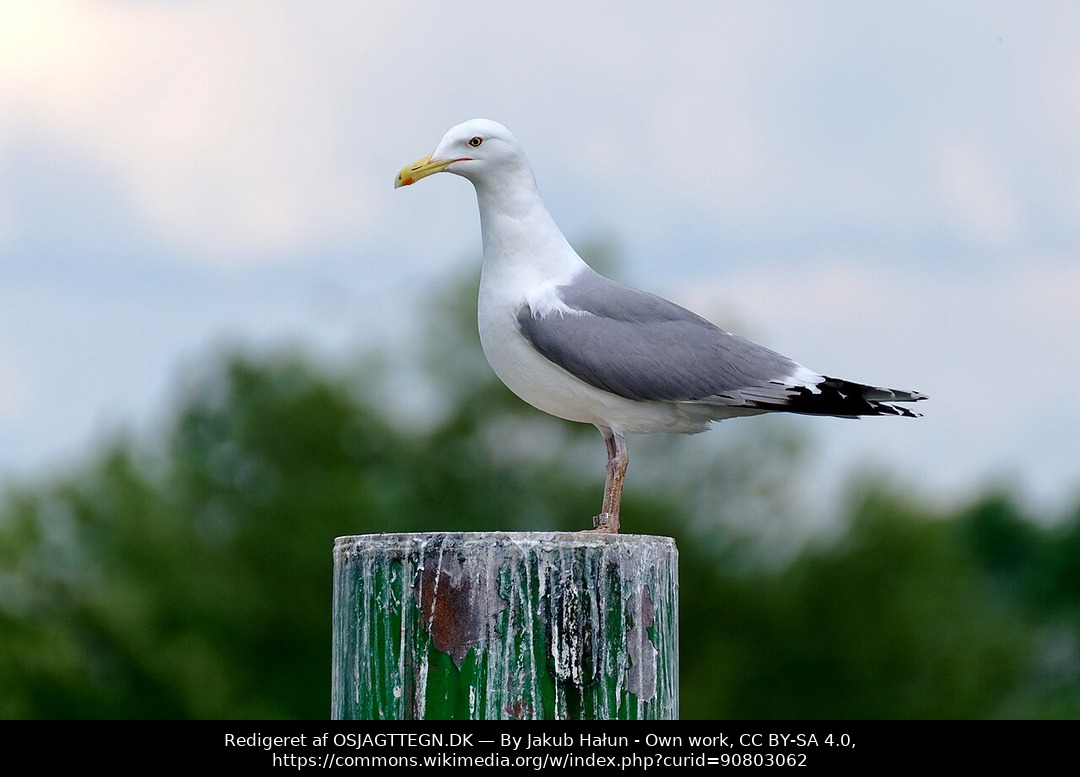
\includegraphics[width=\linewidth, height=7.2cm, keepaspectratio]{Billeder/Dyr/Fugle/Mågefugle/sølvmåge/soelvmaage-01.jpg}
  \end{columns}
\end{frame}
% ========== HÆTTEMÅGE (SOMMERDRAGT) ==========
\begin{frame}{%
  \begin{minipage}[c]{0.30\textwidth}
    Hættemåge\\[-0.1em]
    {\footnotesize (Sommerdragt)}
  \end{minipage}%
  \hfill
  \begin{minipage}[c]{0.45\textwidth}
    \footnotesize
    \textbf{Jagttid:} Ingen jagttid
  \end{minipage}%
  \hfill
  \begin{minipage}[c]{0.15\textwidth}
    \noindent\raggedleft
    
\includegraphics[width=0.5cm, height=0.5cm, keepaspectratio]{Billeder/Ikoner/star.png}
  \end{minipage}%
}
  \vspace{0.25em}
  \begin{columns}[T]
    \column{0.45\textwidth}
    \setlength{\parskip}{0.5em}
    \tiny
    \RaggedRight
    \textbf{\textit{Chroicocephalus ridibundus}} – lille, slank måge med hvidlig vingeforkant \par
    \textbf{Udseende:}\\
    \quad – Mørkebrun hætte som ikke går ned i nakken \\
    \quad – Rødt næb og røde ben \\
    \quad – Hvid krop med grå overside
    \column{0.52\textwidth}
    \centering
    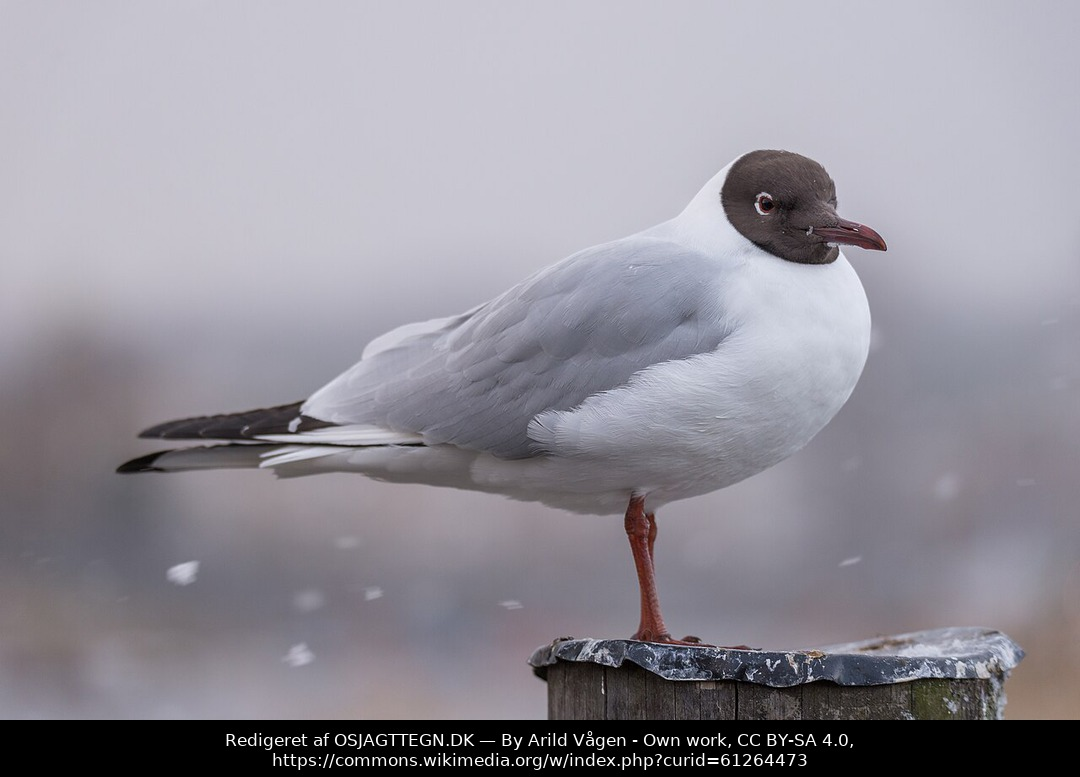
\includegraphics[width=\linewidth, height=7.2cm, keepaspectratio]{Billeder/Dyr/Fugle/Mågefugle/hættemåge/sommer.jpg}
  \end{columns}
\end{frame}

% ========== HÆTTEMÅGE (VINTERDRAGT) ==========
\begin{frame}{%
  \begin{minipage}[c]{0.30\textwidth}
    Hættemåge\\[-0.1em]
    {\footnotesize(Vinterdragt)}
  \end{minipage}%
  \hfill
  \begin{minipage}[c]{0.45\textwidth}
    \footnotesize
    \textbf{Jagttid:} Ingen jagttid
  \end{minipage}%
  \hfill
  \begin{minipage}[c]{0.15\textwidth}
    \noindent\raggedleft
    
\includegraphics[width=0.5cm, height=0.5cm, keepaspectratio]{Billeder/Ikoner/star.png}
  \end{minipage}%
}
  \vspace{0.25em}
  \begin{columns}[T]
    \column{0.45\textwidth}
    \setlength{\parskip}{0.5em}
    \tiny
    \RaggedRight
    \textbf{\textit{Chroicocephalus ridibundus}} – lille, slank måge med hvidlig vingeforkant \par
    \textbf{Udseende:}\\
    \quad – Ingen mørk hætte \\
    \quad – Mørkebrun plet bag øjet \\
    \quad – Hvidt hoved og hvid krop med grå overside
    \column{0.52\textwidth}
    \centering
    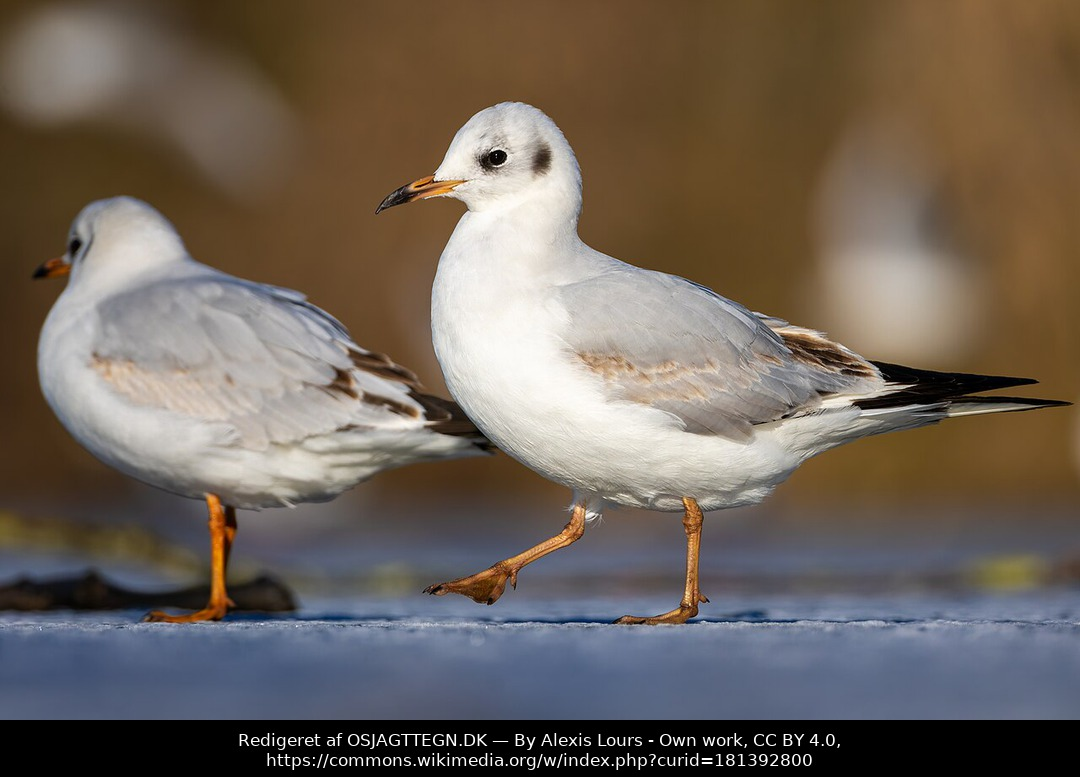
\includegraphics[width=\linewidth, height=7.2cm, keepaspectratio]{Billeder/Dyr/Fugle/Mågefugle/hættemåge/vinter.jpg}
  \end{columns}
\end{frame}
% ========== SILDEMÅGE ==========
\begin{frame}{%
  \begin{minipage}[c]{0.30\textwidth}
    Sildemåge
  \end{minipage}%
  \hfill
  \begin{minipage}[c]{0.45\textwidth}
    \footnotesize
    \textbf{Jagttid:} Ingen jagttid
  \end{minipage}%
  \hfill
  \begin{minipage}[c]{0.15\textwidth}
    \noindent\raggedleft
    
\includegraphics[width=0.5cm, height=0.5cm, keepaspectratio]{Billeder/Ikoner/star.png}
  \end{minipage}%
}
  \vspace{0.25em}
  \begin{columns}[T]
    \column{0.45\textwidth}
    \setlength{\parskip}{0.5em}
    \tiny
    \RaggedRight
    \textbf{\textit{Larus fuscus}} – mellemstor måge der ligner lille svartbag \par
    \textbf{Udseende:}\\
    \quad – Sort/mørk ryg og overvinger \\
    \quad – Hvide pletter på halefjerene \\
    \quad – Gule ben
    \column{0.52\textwidth}
    \centering
    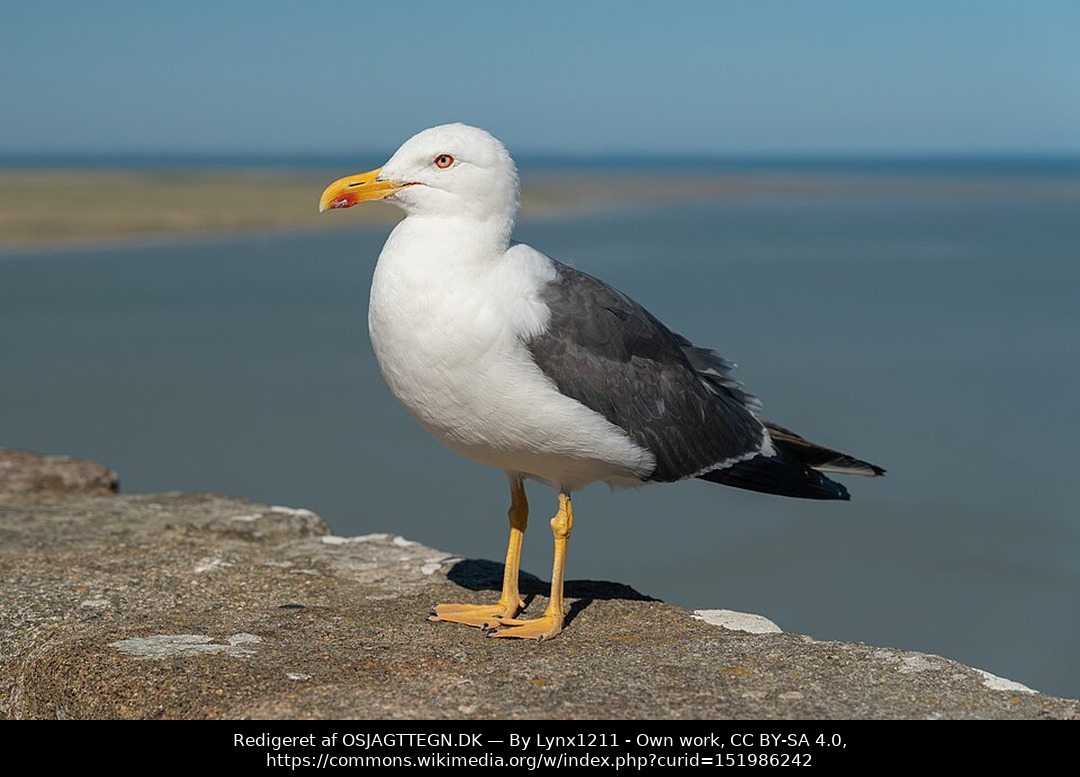
\includegraphics[width=\linewidth, height=7.2cm, keepaspectratio]{Billeder/Dyr/Fugle/Mågefugle/sildemåge/sildemaage-01.jpg}
  \end{columns}
\end{frame}
% ========== STORMMÅGE ==========
\begin{frame}{%
  \begin{minipage}[c]{0.30\textwidth}
    Stormmåge
  \end{minipage}%
  \hfill
  \begin{minipage}[c]{0.45\textwidth}
    \footnotesize
    \textbf{Jagttid:} Ingen jagttid
  \end{minipage}%
  \hfill
  \begin{minipage}[c]{0.15\textwidth}
    \noindent\raggedleft
    
\includegraphics[width=0.5cm, height=0.5cm, keepaspectratio]{Billeder/Ikoner/star.png}
  \end{minipage}%
}
  \vspace{0.25em}
  \begin{columns}[T]
    \column{0.45\textwidth}
    \setlength{\parskip}{0.5em}
    \tiny
    \RaggedRight
    \textbf{\textit{Larus canus}} – lille til mellemstor måge \par
    \textbf{Udseende:}\\
    \quad – Rundt hoved \\
    \quad – Mørkt øje (ser venlig ud) \\
    \quad – Slankt næb
    \column{0.52\textwidth}
    \centering
    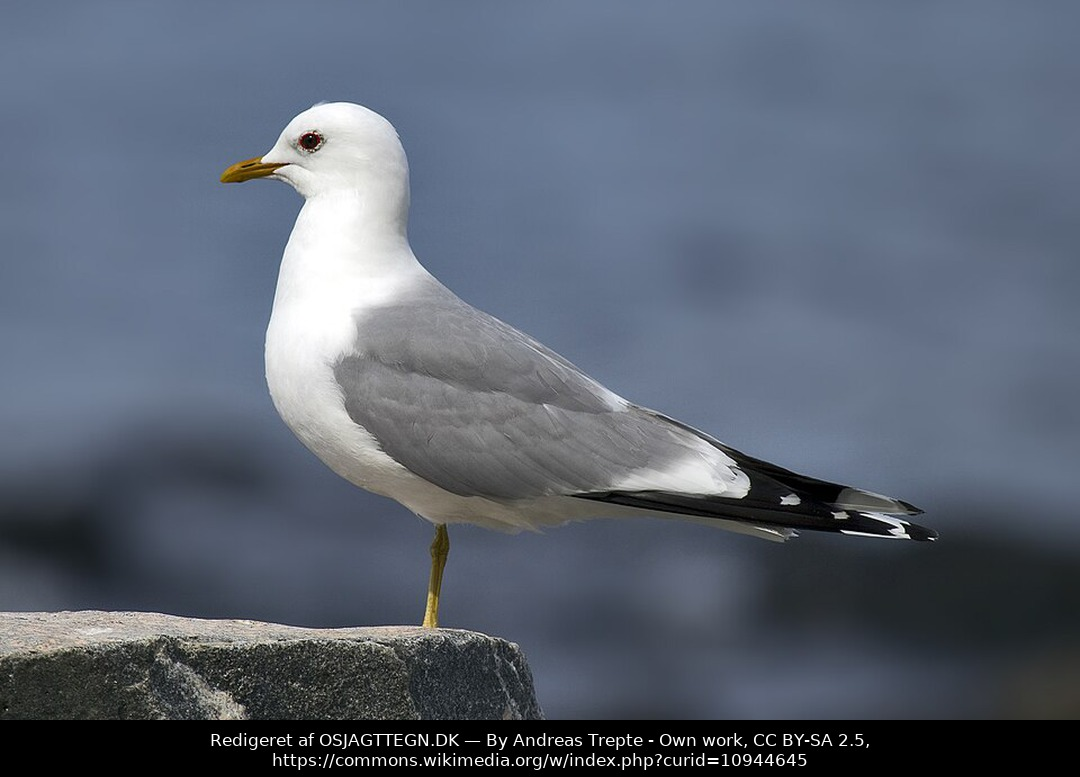
\includegraphics[width=\linewidth, height=7.2cm, keepaspectratio]{Billeder/Dyr/Fugle/Mågefugle/stormmåge/stormmaage-05.jpg}
  \end{columns}
\end{frame}
% ========== SVARTBAG ==========
\begin{frame}{%
  \begin{minipage}[c]{0.30\textwidth}
    Svartbag
  \end{minipage}%
  \hfill
  \begin{minipage}[c]{0.45\textwidth}
    \footnotesize
    \textbf{Jagttid:} Ingen jagttid
  \end{minipage}%
  \hfill
  \begin{minipage}[c]{0.15\textwidth}
    \noindent\raggedleft
    
\includegraphics[width=0.5cm, height=0.5cm, keepaspectratio]{Billeder/Ikoner/star.png}
  \end{minipage}%
}
  \vspace{0.25em}
  \begin{columns}[T]
    \column{0.45\textwidth}
    \setlength{\parskip}{0.5em}
    \tiny
    \RaggedRight
    \textbf{\textit{Larus marinus}} – meget stor og kraftig måge \par
    \textbf{Udseende:}\\
    \quad – Sort ryg og vingeoversider \\
    \quad – Hvide pletter på halen (blinklys) \\
    \quad – Lyserøde ben \\
    \quad – Kraftigt, ``fortrykket'' næb
    \column{0.52\textwidth}
    \centering
    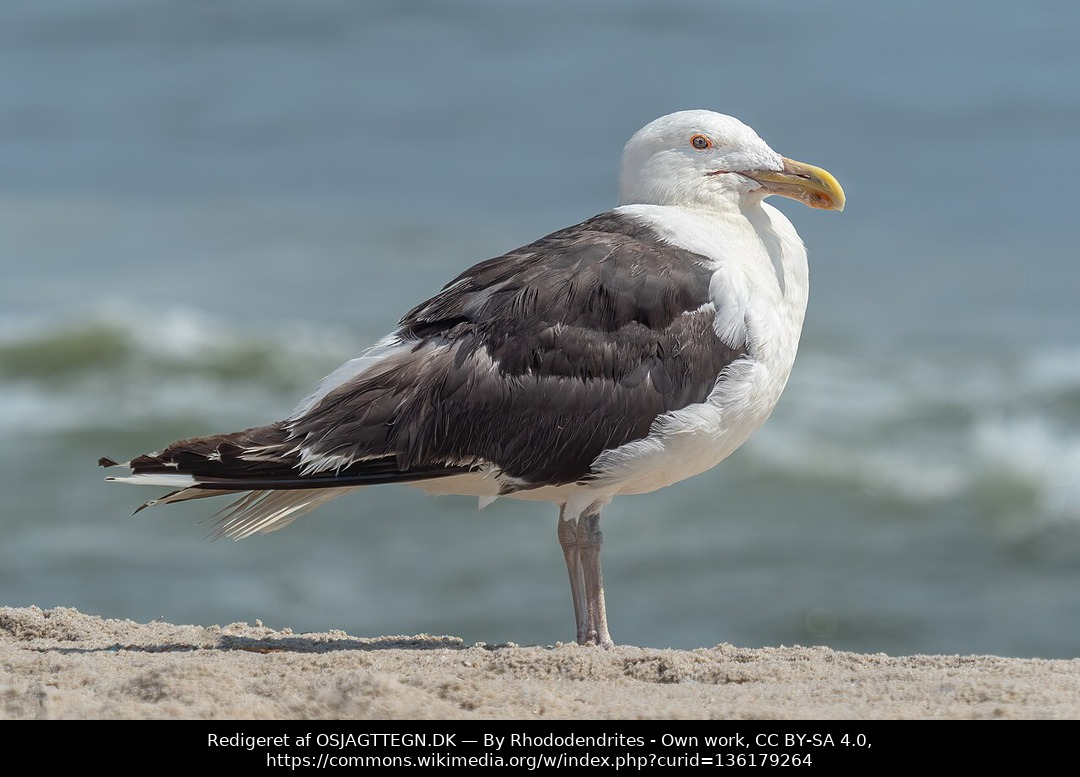
\includegraphics[width=\linewidth, height=7.2cm, keepaspectratio]{Billeder/Dyr/Fugle/Mågefugle/svartbag/svartbag-01.jpg}
  \end{columns}
\end{frame}
\begin{frame}
  \vspace{1.8em}
  \begin{center}
    \begin{minipage}{0.22\textwidth}
      \centering
      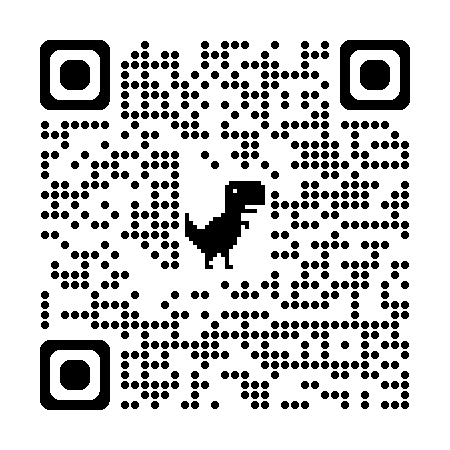
\includegraphics[width=\linewidth]{Billeder/Dyr/Fugle/Mågefugle/qr/maagefugle_qr.png}
    \end{minipage}%
    \hspace{0.8em}%
    \begin{minipage}{0.62\textwidth}
      \raggedright
      \Large
      \textbf{Træning i artsbestemmelse af mågefugle}\\[0.35em]
      {\large https://osjagttegn.dk/maagefugle}
    \end{minipage}
  \end{center}
\end{frame}